\chapter{Continuous Probability Models}  
\label{chap:contin}

There are other types of random variables besides the discrete ones you
studied in Chapter \ref{dis}.  This chapter will cover another major
class, {\it continuous random variables}, which form the heart of
statistics and are used extensively in applied probability as well.  It
is for such random variables that the calculus prerequisite for this
book is needed.

\section{Running Example:  a Random Dart}
\label{dart}

Imagine that we throw a dart at random at the interval (0,1).  Let D
denote the spot we hit.  By ``at random'' we mean that all subintervals
of equal length are equally likely to get hit.  For instance, the
probability of the dart landing in (0.7,0.8) is the same as for
(0.2,0.3), (0.537,0.637) and so on.

Because of that randomness, 

\begin{equation}
\label{vminusu}
P(u \leq D \leq v) = v-u
\end{equation}

for any case of $0 \leq u < v \leq 1$.

We call D a {\bf continuous} random variable, because its support is a
continuum of points, in this case, the entire interval (0,1).

\section{Individual Values Now Have Probability Zero}

The first crucial point to note is that 

\begin{equation}
\label{itszero}
P(D = c) = 0
\end{equation}

for any individual point c.  This may seem counterintuitive, but it can
be seen in a couple of ways:

\begin{itemize}

\item Take for example the case c = 0.3.  Then

\begin{equation}
\label{1921}
P(D = 0.3) \leq P( 0.29 \leq D \leq 0.31) = 0.02
\end{equation}

the last equality coming from (\ref{vminusu}).  

So, $P(D = 0.3) \leq 0.02$.  But we can replace 0.29 and 0.31 in
(\ref{1921}) by 0.299 and 0.301, say, and get $P(D = 0.3) \leq 0.002$.  
So, $P(D = 0.3)$ must be smaller than any positive number, and thus it's
actually 0.

\item Reason that there are infinitely many points, and if they all had
some nonzero probability w, say, then the probabilities would sum to
infinity instead of to 1; thus they must have probability 0.

\end{itemize}

Similarly, one will see that (\ref{itszero}) will hold for any
continuous random variable.

Remember, we have been looking at probability as being the long-run
fraction of the time an event occurs, in infinitely many repetitions of
our experiment---the ``notebook'' view.  So (\ref{itszero}) doesn't say
that D = c can't occur; it merely says that it happens so rarely that
the long-run fraction of occurrence is 0. 

\section{But Now We Have a Problem}
\label{presentsaproblem}

But Equation (\ref{itszero}) presents a problem.  In the case of
discrete random variables M, we defined their distribution via their
probability mass function, $p_M$.  Recall that Section \ref{dstrdef}
defined this as a list of the values M takes on, together with their
probabilities.  But that would be impossible in the continuous
case---all the probabilities of individual values here are 0.

So our goal will be to develop another kind of function, which is
similar to probability mass functions in spirit, but circumvents the
problem of individual values having probability 0.  To do this, 
we first must define another key function:

\subsection{Our Way Out of the Problem:  Cumulative Distribution Functions}
\label{cdfdef}

\begin{definition}
For any random variable W (including discrete ones),
its {\bf cumulative distribution function} (cdf), $F_W$, is defined by

\begin{equation}
\label{cdf}
F_W(t) = P(W \leq t), -\infty < t < \infty
\end{equation}
\end{definition}

(Please keep in mind the notation.  It is customary to use capital F to
denote a cdf, with a subscript consisting of the name of the random
variable.)

What is t here?  It's simply an argument to a function.  The function
here has domain $(-\infty, \infty)$, and we must thus define that
function for every value of t.  This is a simple point, but a crucial
one.

For an example of a cdf, consider our ``random dart'' example above.  We
know that, for example for t = 0.23,

\begin{equation}
F_D(0.23) = P(D \leq 0.23) = P(0 \leq D \leq 0.23) = 0.23
\end{equation}

Also, 

\begin{equation}
F_D(-10.23) = P(D \leq -10.23) = 0
\end{equation}

and

\begin{equation}
F_D(10.23) = P(D \leq 10.23) = 1
\end{equation}

Note that {\it the fact that D can never be equal to 10.23 or anywhere
near it is irrelevant}.  $F_D(t)$ is defined for {\it all} t in
$(-\infty,\infty)$, including 10.23!  The definition of $F_D(10.23)$ is
$P(D \leq 10.23))$, and that probability is 1!  Yes, D is {\it always}
less than or equal to 10.23, right?

In general for our dart,

\begin{equation}
\label{unifcdf}
F_D(t) = 
\begin{cases}
0, & \text{if $t \leq 0$} \\
t, & \text{if $0 < t < 1$} \\ 
1, & \text{if $t \geq 1$} \\
\end{cases}
\end{equation}

Here is the graph of $F_D$: 

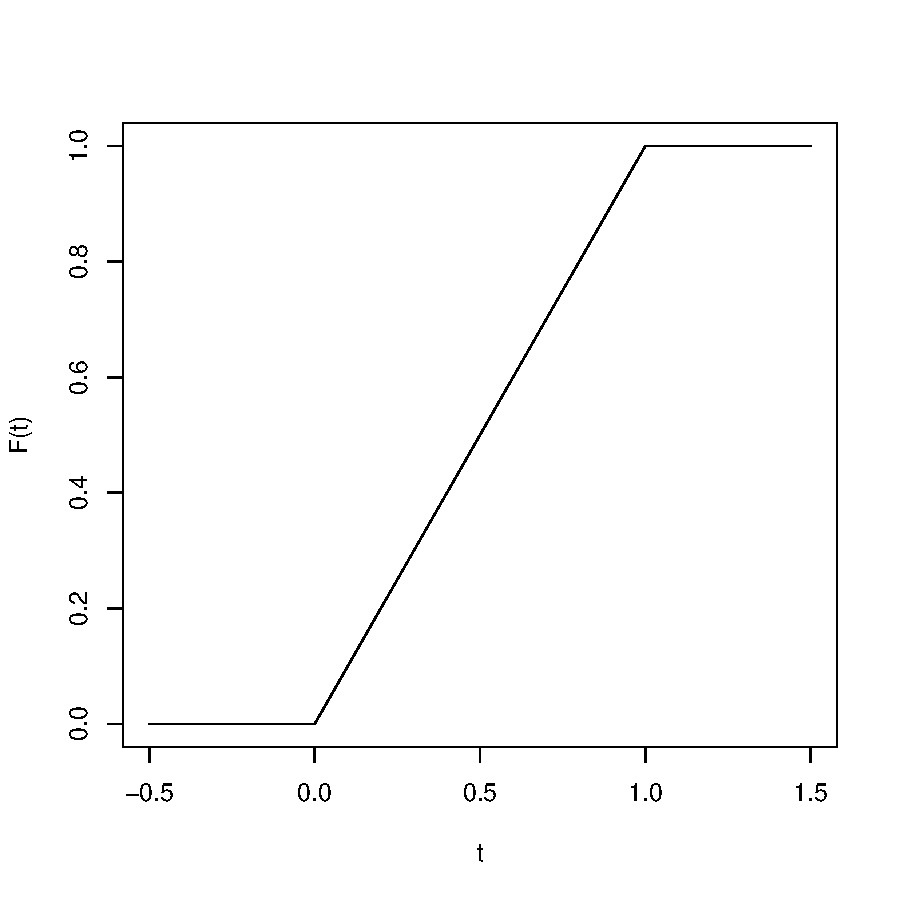
\includegraphics[width=3.5in]{FD.pdf}

The cdf of a discrete random variable is defined as in Equation
(\ref{cdf}) too.  For example, say Z is the number of heads we get from
two tosses of a coin.  Then

\begin{equation}
\label{binomcdf}
F_Z(t) =
\begin{cases}
0, & \text{if $t <  0$} \\
0.25, & \text{if $0 \leq t <  1$} \\
0.75, & \text{if $1 \leq t <  2$} \\
1, & \text{if $t \geq 2$} \\
\end{cases}
\end{equation}

For instance, 

\begin{eqnarray}
F_Z(1.2) &=& P(Z \leq 1.2) \\ 
&=& P(Z = 0 \textrm{ or } Z = 1) \label{z01} \\
&=& 0.25 + 0.50 \label{binom2575} \\
&=& 0.75
\end{eqnarray}

Note that (\ref{z01}) is simply a matter of asking our famous question,
``How can it happen?''  Here we are asking how it can happen that $Z
\leq 1.2$.  The answer is simple:  That can happen if Z is 0 or 1.  {\it
The fact that Z cannot equal 1.2 is irrelevant.}

(\ref{binom2575}) uses the fact that Z has a binomial
distribution with n = 2 and p = 0.5.

$F_Z$ is graphed below.  

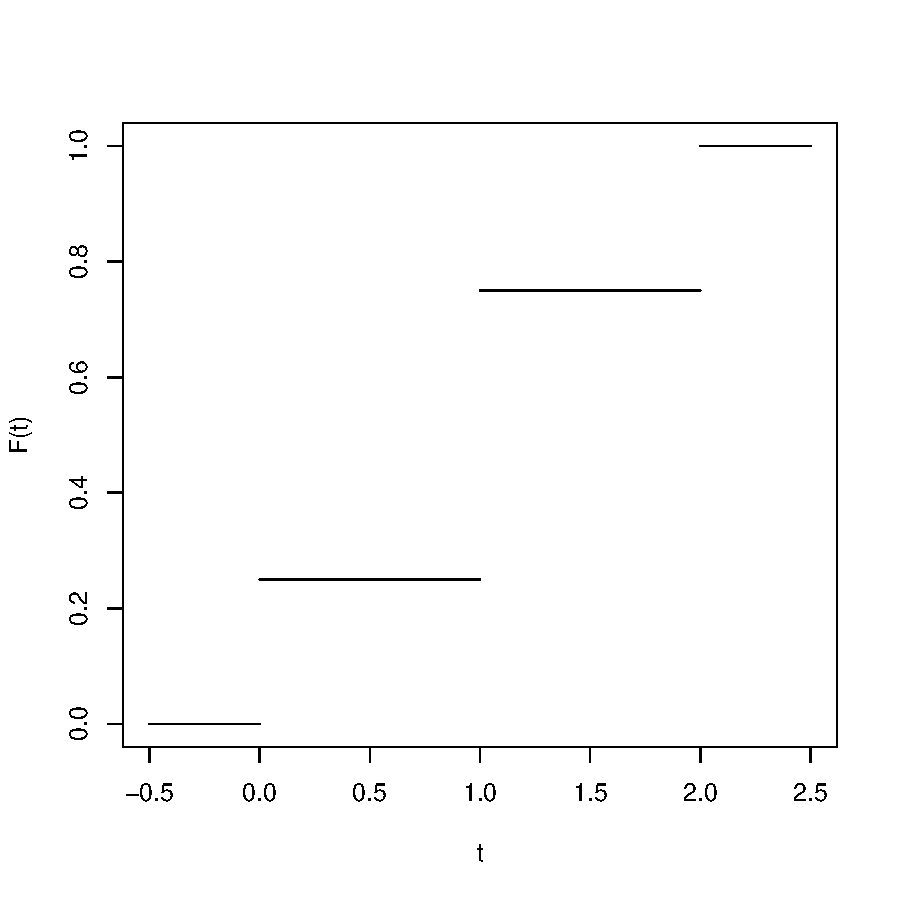
\includegraphics[width=4in]{FZ.pdf}

The fact that one cannot get a noninteger number of heads is what makes
the cdf of Z flat between consecutive integers.          

In the graphs you see that $F_D$ in (\ref{unifcdf}) is continuous while
$F_Z$ in (\ref{binomcdf}) has jumps.  This is another reason we call
random variables such as D {\bf continuous random variables}. 

% Students sometimes ask, ``What is t?"  The answer is that it's simply
% the argument of a mathematical function, just like the role of t in,
% say, $g(t) = sin(\pi t), -\infty < t < \infty$.  $F_Z()$ is a function,
% just like this g(t) or the numerous functions that you worked with in
% calculus.  Each input yields an ouput; the input 1.2 yields the output
% 0.75 in the case of $F_Z()$ while the input 1 yields the output 0 in the
% case of g(t).

At this level of study of probability, random variables are either
discrete or continuous.  But some exist that are neither.  We won't see
any random variables from the ``neither'' case here, and they occur
rather rarely in practice.

Armed with cdfs, let's turn to the original goal, which was to find
something for continuous random variables that is similar in spirit to
probability mass functions for discrete random variables.

\subsection{Density Functions}
\label{densitymotivation}

{\fbox {\parbox{6.5in}{
Intuition is key here.  Make SURE you develop a good intuitive 
understanding of density functions, as it is vital in being able to 
apply probability well.  We will use it a lot in our course.  
}}}

(The reader may wish to review pmfs in Section \ref{dstrdef}.)

Think as follows.  From (\ref{cdf}) we can see that for a discrete
random variable, its cdf can be calculated by summing its pmf.  Recall
that in the continuous world, we integrate instead of sum.
So, our continuous-case analog of the pmf should be
something that integrates to the cdf.  That of course is the derivative
of the cdf, which is called the {\bf density}:  

\begin{definition} 
Consider a continuous random variable W.  Define

\begin{equation}
\label{dens}
f_W(t) = \frac{d}{dt} F_W(t), -\infty < t < \infty
\end{equation}

wherever the derivative exists.  The function $f_W$ is called the {\bf
probability density function} (pdf), or just the {\bf density} of W.
\end{definition}

(Please keep in mind the notation.  It is customary to use lower-case f
to denote a density, with a subscript consisting of the name of the
random variable.)

But what {\it is} a density function?  First and foremost, it is a tool
for finding probabilities involving continuous random variables:

\subsection{Properties of Densities}

Equation (\ref{dens}) implies 

{\bf Property A:}

\begin{eqnarray}
\label{ntab}
P(a < W \leq b) &=& F_W(b) - F_W(a) \\
&=& \int_{a}^{b} f_W(t) ~ dt \label{ftc}
\end{eqnarray}

Where does (\ref{ntab}) come from?  Well, $F_W(b)$ is all the
probability accumulated from $-\infty$ to $b$, while $F_W(a)$ is all the
probability accumulated from $-\infty$ to $a$.  The difference is the
probability that X is {\it between} $a$ and $b$.

(\ref{ftc}) is just the Fundamental Theorem of Calculus:  Integrate the
derivative of a function, and you get the original function back again.

Since P(W = c) = 0 for any single point c, Property A also means:

{\bf Property B:}

\begin{equation}
P(a < W \leq b) = 
P(a \leq W \leq b) = 
P(a \leq W < b) = 
P(a < W < b) = 
\int_{a}^{b} f_W(t) ~ dt
\end{equation}

This in turn implies: 

{\bf Property C:}

\begin{equation}
\label{total1}
\int_{-\infty}^{\infty} f_W(t) ~ dt = 1
\end{equation}

Note that in the above integral, $f_W(t)$ will be 0 in various ranges of
t corresponding to values W cannot take on.  For the dart example, for
instance, this will be the case for $t < 0$ and $t > 1$.

Any nonnegative function that integrates to 1 is a density.  A density
could be increasing, decreasing or mixed.  Note too that a density can
have values larger than 1 at some points, even though it must integrate
to 1.  

\subsection{Intuitive Meaning of Densities}

Suppose we have some continuous random variable X, with density $f_X$,
graphed in Figure \ref{pm}.

Let's think about probabilities of the form 

\begin{equation}
P(s - 0.1 < X < s + 0.1)
\end{equation}

Let's first consider the case of s = 1.3.

The rectangular strip in the picture should remind you of your early
days in calculus.  What the picture says is that the area under $f_X$
from 1.2 to 1.4 (i.e.\ $1.3 \pm 0.1$) is approximately equal to the area
of the rectangle.  In other words,

\begin{equation}
2 (0.1) f_X(1.3) \approx \int_{1.2}^{1.4} f_X(t) ~ dt 
\end{equation}

But from our Properties above, we can write this as

\begin{equation}
\label{eq124}
P(1.2 < X < 1.4) \approx 2 (0.1) f_X(1.3) 
\end{equation}

Similarly, for s = 0.4,

\begin{equation}
\label{eq035}
P(0.3 < X < 0.5) \approx 2 (0.1) f_X(0.4) 
\end{equation}

and in general

\begin{equation}
\label{equuu}
P(s-0.1 < X < s+0.1) \approx 2 (0.1) f_X(s) 
\end{equation}

This reasoning shows that:

\begin{quote}
Regions in the number line (X-axis in the picture)
with low density have low probabilities while regions with high
density have high probabilities.  
\end{quote}

So, although densities themselves are not probabilities, they do tell us
which regions will occur often or rarely.  For the random variable X in
our picture, there will be many lines in the notebook in which X is near
1.3, but many fewer in which X is near 0.4.

\begin{figure}
\centerline{
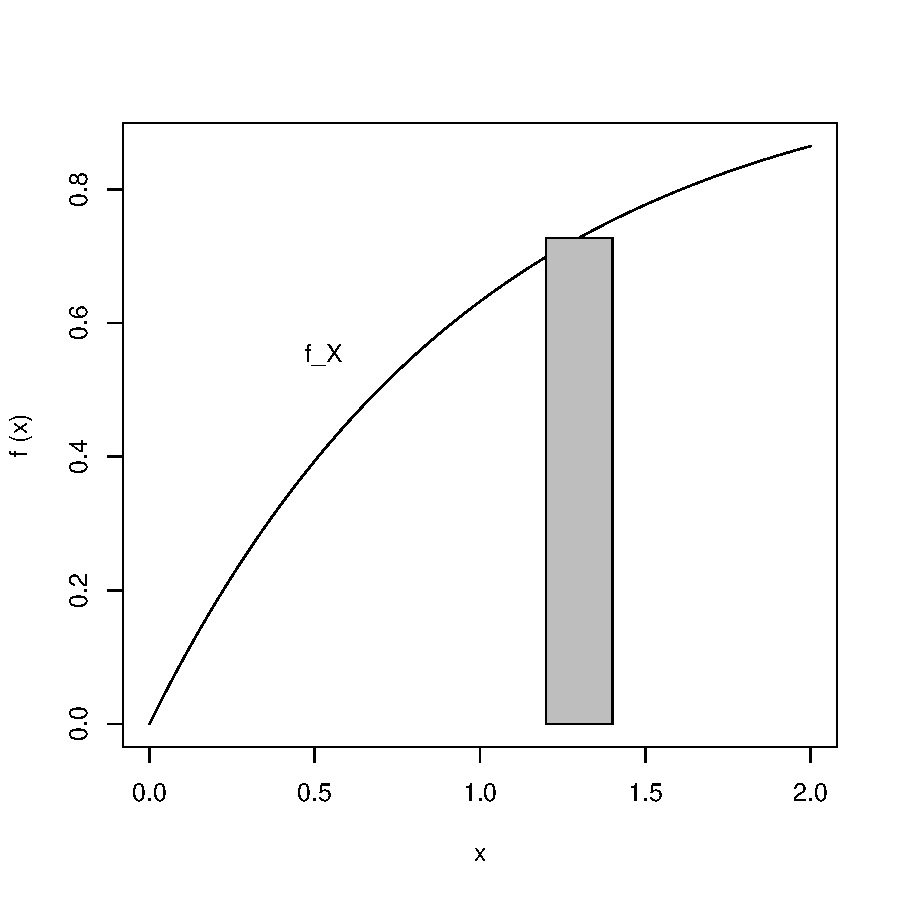
\includegraphics[width=4in]{PlusMinusC.pdf}
}
\caption{Approximation of Probability by a Rectangle}
\label{pm}
\end{figure}

\subsection{Expected Values}

What about E(W)?  Recall that if W were discrete, we'd have 

\begin{equation}
E(W) = \sum_{c} c p_W(c)
\end{equation}

where the sum ranges overall all values c that W can take on.  If for
example W is the number of dots we get in rolling two dice, c will range
over the values 2,3,...,12.

So, the analog for continuous W is:

{\bf Property D:}

\begin{equation}
E(W) = \int_t t f_W(t) ~ dt
\end{equation}

where here t ranges over the values W can take on, such as the interval
(0,1) in the dart case.  Again, we can also write this as

\begin{equation}
E(W) = \int_{-\infty}^{\infty}  t f_W(t) ~ dt
\end{equation}

in view of the previous comment that $f_W(t)$ might be 0 for various
ranges of t.

And of course, 

\begin{equation}
E(W^2) = \int_t t^2 f_W(t) ~ dt
\end{equation}

and in general, similarly to (\ref{egofx}):

{\bf Property E:}

\begin{equation}
\label{eofgofw}
E[g(W)] = \int_t g(t) f_W(t) ~ dt
\end{equation}

Most of the properties of expected value and variance stated previously
for discrete random variables hold for continuous ones too:

{\bf Property F:}

Equations (\ref{eofsum}), (\ref{aubv}), (\ref{factoring}),
(\ref{varuformula}) and (\ref{varcu}) still hold in the
continuous case.

\section{A First Example}
\label{afirstex}

Consider the density function equal to 2t/15 on the
interval (1,4), 0 elsewhere.  Say X has this density.  Here are some
computations we can do: 

\begin{equation}
\label{ex2t15}
EX = \int_{1}^{4} t \cdot 2t/15 ~ dt = 2.8
\end{equation}

\begin{equation}
P(X > 2.5) = \int_{2.5}^{4} 2t/15 ~ dt = 0.65
\end{equation}

\begin{equation}
F_X(s) = \int_{1}^{s} 2t/15 ~ dt = \frac{s^2-1}{15} ~~~~ \textrm{for s in
(1,4) (cdf is 0 for t $<$ 1, and 1 for t $>$ 4)}
\end{equation}

\begin{eqnarray}
Var(X) &=& E(X^2) - (EX)^2 ~~~~ \textrm{(from (\ref{varuformula})}\\ 
&=& \int_{1}^{4} t^2 2t/15 ~ dt - 2.8^2 ~~~~ \textrm{(from (\ref{ex2t15}))} \\
&=& 0.66
\end{eqnarray}

% \begin{eqnarray}
% P(\textrm{tenths digit of X is even}) 
% &=& \sum_{i=0}^{28} 
% P \left [ 1+i/10 < X < 1+(i+1)/10 \right ] \\
% &=& \sum_{i=0}^{28}
% \int_{1+i/10}^{1+(i+1)/10} 2t/15 ~ dt \\
% &=& ... \textrm{ (integration left to the reader)}
% \end{eqnarray}

Suppose L is the lifetime of a light bulb (say in years), with the
density that X has above.  Let's find some quantities in that context:

{\bf  Proportion of bulbs with lifetime less than
the mean lifetime:}

\begin{equation}
P(L < 2.8) = \int_{1}^{2.8} 2t/15 ~ dt = (2.8^2 - 1)/15
\end{equation}

{\bf Mean of 1/L:}

\begin{equation}
E(1/L) = \int_{1}^{4} \frac{1}{t} \cdot 2t/15 ~ dt = \frac{2}{5}
\end{equation}

{\bf In testing many bulbs, mean number of bulbs that it takes to find
two that have lifetimes longer than 2.5:}

Use (\ref{negbinpmf}) with r = 2 and p = 0.65.

\section{The Notion of {\it Support} in the Continuous Case}
\label{continsupport}

Recall from Section \ref{support} that the {\it support} of a discrete
distribution is its ``domain.''  If for instance X is the number of
heads I get from 3 tosses of a coin, X can only take on the values 0, 1,
2 and 3.  We say that that set is the support of this distribution; 8,
for example, is not in the support.

The notion extends to continuous random variables.  In Section
\ref{afirstex}, the support of the density there is the interval (1,4).

\section{Famous Parametric Families of Continuous Distributions}

\subsection{The Uniform Distributions}

\subsubsection{Density and Properties}
\label{unifprops} 

In our dart example, we can imagine throwing the dart at the interval
(q,r) (so this will be a two-parameter family).  Then to be a uniform
distribution, i.e. with all the points being ``equally likely,'' the
density must be constant in that interval.  But it also must integrate
to 1 [see (\ref{total1}).  So, that constant must be 1 divided by the
length of the interval:

\begin{equation}
f_D(t) = \frac{1}{r-q} 
\end{equation}

for t in (q,r), 0 elsewhere.  

It easily shown that $E(D) = \frac{q+r}{2}$ and $Var(D) = \frac{1}{12} (r-q)^2$.

The notation for this family is U(q,r).

\subsubsection{R Functions}

Relevant functions for a uniformly  distributed random variable X 
on (r,s) are:

\begin{itemize}

\item {\bf dunif(x,r,s)}, to find $f_X(x)$

\item {\bf punif(q,r,s)}, to find $P(X \leq q)$

\item {\bf qunif(q,r,s)}, to find c such that $P(X \leq c) = q$

\item {\bf runif(n,r,s)}, to generate n independent values of X

\end{itemize}

As with most such distribution-related functions in R, {\bf x} and {\bf
q} can be vectors, so that {\bf punif()} for instance can be used to
find the cdf values at multiple points.

\subsubsection{Example:  Modeling of Disk Performance}

Uniform distributions are often used to model computer disk requests.
Recall that a disk consists of a large number of concentric rings,
called {\bf tracks}.  When a program issues a request to read or write a
file, the {\bf read/write head} must be positioned above the track of
the first part of the file.  This move, which is called a {\bf seek},
can be a significant factor in disk performance in large systems, e.g. a
database for a bank.

\label{defrag}
If the number of tracks is large, the position of the read/write head,
which I'll denote as X, is like a continuous random variable, and 
often this position is modeled by a uniform distribution.  This 
situation may hold just before a defragmentation operation.  After 
that operation, the files tend to be bunched together in the central 
tracks of the disk, so as to reduce seek time, and X will not have a
uniform distribution anymore.

Each track consists of a certain number of {\bf sectors} of a given
size, say 512 bytes each.  Once the read/write head reaches the proper
track, we must wait for the desired sector to rotate around and pass
under the read/write head.  It should be clear that a uniform
distribution is a good model for this {\bf rotational delay}.

For example, suppose in modeling disk performance, we describe the
position X of the read/write head as a number between 0 and 1,
representing the innermost and outermost tracks, respectively.  Say we
assume X has a uniform distribution on (0,1), as discussed above.
Consider two consecutive positions (i.e.  due to two consecutive seeks),
$X_1$ and $X_2$, which we'll assume are independent.\footnote{NOT a good
assumption for consecutive seeks; think about why.} Let's find $Var(X_1
+ X_2)$.

We know from Section \ref{unifprops} that the variance of a U(0,1)
distribution is 1/12.  Then by independence,

\begin{equation}
Var(X_1 + X_2) = 1/12 + 1/12 = 1/6
\end{equation}

\subsubsection{Example:  Modeling of Denial-of-Service Attack}

In one facet of computer security, it has been found that a uniform
distribution is actually a warning of trouble, a possible indication of
a {\bf denial-of-service attack}.  Here the attacker tries to
monopolize, say, a Web server, by inundating it with service requests.
According to the research of David Marchette,\footnote{{\it Statistical
Methods for Network and Computer Security}, David J. Marchette, Naval
Surface Warfare Center,
\url{rion.math.iastate.edu/IA/2003/foils/marchette.pdf}.} attackers
choose uniformly distributed false IP addresses, a pattern not normally
seen at servers.

\subsection{The Normal (Gaussian) Family of Continuous Distributions}  
\label{normalfam}

These are the famous ``bell-shaped curves,'' so called because their
densities have that shape.\footnote{{\it All that glitters is not
gold''}---Shakespeare

Note that other parametric families, notably the Cauchy, also have bell
shapes.  The difference lies in the rate at which the tails of the
distribution go to 0.  However, due to the Central Limit Theorem, to be
presented below, the normal family is of prime interest.}

\subsubsection{Density and Properties}

{\bf Density and Parameters:}

The density for a normal distribution is

\begin{equation}
f_W(t) = \frac{1}{\sqrt{2\pi} \sigma} ~ e^{- 0.5 \left (\frac{t-\mu}{\sigma}
\right )^2}, -\infty < t < \infty
\end{equation}

Again, this is a two-parameter family, indexed by the parameters $\mu$
and $\sigma$, which turn out to be the mean\footnote{Remember, this is a
synonym for expected value.} and standard deviation  $\mu$ and $\sigma$,
The notation for it is $N(\mu,\sigma^2)$ (it is customary to state
the variance $\sigma^2$ rather than the standard deviation).

The normal family is so important that we have a special chapter on it,
Chapter \ref{chap:normal}.

\subsection{The Exponential Family of Distributions}
\label{exponfam}

Please note:  We have been talking here of parametric families of
distributions, and in this section will introduce one of the most
famous, the family of exponential distributions.  This should not be
confused, though, with the term {\it exponential family} that arises in
mathematical statistics, which includes exponential distributions but is
much broader.

\subsubsection{Density and Properties}
\label{expon}

The densities in this family have the form

\begin{equation}
\label{expdens}
f_W(t) = \lambda e^{-\lambda t}, 0 < t < \infty
\end{equation}

This is a one-parameter family of distributions. 

After integration, one finds that $E(W) = \frac{1}{\lambda}$ and $Var(W)
= \frac{1}{\lambda^2}$.  You might wonder why it is customary to index
the family via $\lambda$ rather than $1/\lambda$ (see (\ref{expdens})),
since the latter is the mean.  But this is actually quite natural, for
reasons discussed in Section \ref{connpoi}.

\subsubsection{R Functions}

Relevant functions for a uniformly  distributed random variable X 
with parameter $\lambda$ are

\begin{itemize}

\item {\bf dexp(x,lambda)}, to find $f_X(x)$

\item {\bf pexp(q,lambda)}, to find $P(X \leq q)$

\item {\bf qexp(q,lambda)}, to find c such that $P(X \leq c) = q$

\item {\bf rexp(n,lambda)}, to generate n independent values of X

\end{itemize}

\subsubsection{Example:  Refunds on Failed Components}

Suppose a manufacturer of some electronic component finds that its
lifetime L is exponentially distributed with mean 10000 hours. They give a
refund if the item fails before 500 hours. Let $M$ be the number of items
they have sold, up to and including the one on which they make the first
refund. Let's find $EM$ and $Var(M)$.  

First, notice that $M$ has a geometric distribution!  It is the number of
independent trials until the first success, where a ``trial'' is one component,
``success'' (no value judgment, remember) is giving a refund, and the
success probability is

\begin{equation}
P(L < 500) = \int_{0}^{500} 0.0001 e^{-0.0001 t} ~ dt = 0.05
\end{equation}

Then plug p = 0.05 into (\ref{meangeom}) and (\ref{vargeom}). 

\subsubsection{Example:  Garage Parking Fees}

A certain public parking garage charges parking fees of \$1.50 for the
first hour, and \$1 per hour after that.  (It is assumed here for
simplicity that the time is prorated within each of those defined
periods.  The reader should consider how the analysis would change if
the garage ``rounds up'' each partial hour.) Suppose parking times T are
exponentially distributed with mean 1.5 hours.  Let W denote the total
fee paid.  Let's find E(W) and Var(W).

The key point is that W is a function of T:

\begin{equation}
\label{ag}
W = 
\begin{cases}
1.5 T, & \text{if $T \leq 1$} \\
1.5 + 1 \cdot (T-1) = T + 0.5, & \text{if $T > 1$} 
\end{cases}
\end{equation}

That's good, because we know how to find the expected value of a
function of a continuous random variable, from (\ref{eofgofw}).
Defining g() as in (\ref{ag}) above, we have

\begin{equation}
EW = \int_{0}^{\infty} g(t) ~ \frac{1}{1.5} e^{-\frac{1}{1.5}t} dt
= \int_{0}^{1} 1.5 t ~ \frac{1}{1.5} e^{-\frac{1}{1.5}t} dt +
\int_{1}^{\infty} (t+0.5) ~ \frac{1}{1.5} e^{-\frac{1}{1.5}t} dt
\end{equation}

The integration is left to the reader.

Now, what about Var(W)?  As is often the case, it's easier to use
(\ref{varuformula}), so we need to find $E(W^2)$.  The above integration
becomes

\begin{equation}
E(W^2) 
= \int_{0}^{\infty} g^2(t) ~ f_W (t) dt
= \int_{0}^{1} t^2 1.5 t ~ \frac{1}{1.5} e^{-\frac{1}{1.5}t} dt +
  \int_{1}^{\infty} (t+0.5)^2 ~ \frac{1}{1.5} e^{-\frac{1}{1.5}t} dt
\end{equation}

After evaluating this, we subtract $(EW)^2$, giving us the variance of
W.

\subsubsection{Importance in Modeling}

Many distributions in real life have been found to be approximately
exponentially distributed.  A famous example is the lifetimes of air
conditioners on airplanes.  Another famous example is interarrival
times, such as customers coming into a bank or messages going out onto a
computer network.  It is used in software reliability studies too.

One of the reasons why this family is used so widely in probabilistic
modeling is that it has several remarkable properties, so many that we
have a special chapter for this family, Chapter \ref{chap:expondistr}.

\subsection{The Gamma Family of Distributions}
\label{gammafam}

\subsubsection{Density and Properties}
\label{gammaprops}

Suppose at time 0 we install a light bulb in a lamp, which burns $X_1$
amount of time.  We immediately install a new bulb then, which burns for
time $X_2$, and so on.  Assume the $X_i$ are independent random
variables having an exponential distribution with parameter $\lambda$.

Let 

\begin{equation}
T_r = X_1 + ... + X_r, ~~ r = 1,2,3,...
\end{equation}

Note that the random variable $T_r$ is the time of the $r^{th}$ light
bulb replacement.  $T_r$ is the sum of r independent exponentially
distributed random variables with parameter $\lambda$.  The distribution
of $T_r$ is called an {\bf Erlang} distribution.  Its density can be
shown to be

\begin{equation}
\label{erldens}
f_{T_r}(t) = \frac{1}{(r-1)!} \lambda^r t^{r-1} e^{-\lambda t}, ~ t > 0
\end{equation}

This is a two-parameter family.

Again, it's helpful to think in ``notebook'' terms.  Say r = 8.  Then we
watch the lamp for the durations of eight lightbulbs, recording $T_8$,
the time at which the eighth burns out.  We write that time in the first
line of our notebook.  Then we watch a new batch of eight bulbs, and
write the value of $T_8$ for those bulbs in the second line of our
notebook, and so on.  Then after recording a very large number of lines
in our notebook, we plot a histogram of all the $T_8$ values.  The point
is then that that histogram will look like (\ref{erldens}).

We can generalize this by allowing r to take noninteger values, by
defining a generalization of the factorial function:

\begin{equation}
\Gamma(r) = \int_{0}^{\infty} x^{r-1} e^{-x}  ~ dx
\end{equation}

This is called the gamma function, and it gives us the gamma family of
distributions, more general than the Erlang:

\begin{equation}
f_W(t) = \frac{1}{\Gamma(r)} \lambda^r t^{r-1} e^{-\lambda t}, ~ t > 0
\end{equation}

(Note that $\Gamma(r)$ is merely serving as the constant that makes the
density integrate to 1.0.  It doesn't have meaning of its own.)

This is again a two-parameter family, with r and $\lambda$ as
parameters.

A gamma distribution has mean $r/\lambda$ and variance $r/\lambda^2$.
In the case of integer r, this follows from (\ref{ti}) and the fact that
an exponentially distributed random variable has mean and variance
$1/\lambda$ and variance $1/\lambda^2$, and it can be derived in
general.  Note again that the gamma reduces to the exponential when r =
1.  

\subsubsection{Example:  Network Buffer}
\label{netbuff}

Suppose in a network context (not our ALOHA example), a node does not
transmit until it has accumulated five messages in its buffer. Suppose
the times between message arrivals are independent and  exponentially
distributed with mean 100 milliseconds.  Let's find the probability that
more than 552 ms will pass before a transmission is made, starting with
an empty buffer. 

Let $X_1$ be the time until the first message arrives, $X_2$ the time
from then to the arrival of the second message, and so on.  Then the
time until we accumulate five messages is $Y = X_1+...+X_5$.  Then from
the definition of the gamma family, we see that Y has a gamma
distribution with r = 5 and $\lambda = 0.01$.  Then

\begin{equation}
P(Y > 552) = 
\int_{552}^{\infty}
\frac{1}{4!} 0.01^5 t^4 e^{-0.01t} ~ dt
\end{equation}

This integral could be evaluated via repeated integration by parts, but
let's use R instead:

\begin{Verbatim}[fontsize=\relsize{-2}]
> 1 - pgamma(552,5,0.01)
[1] 0.3544101
\end{Verbatim}

Note that our parameter r is called {\bf shape} in R, and our $\lambda$
is {\bf rate}.

Again, there are also {\bf dgamma()}, {\bf qgamma()} and {\bf rgamma()}.
From the R man page:

\begin{lstlisting}
Usage:

     dgamma(x, shape, rate = 1, scale = 1/rate, log = FALSE)
     pgamma(q, shape, rate = 1, scale = 1/rate, lower.tail = TRUE,
            log.p = FALSE)
     qgamma(p, shape, rate = 1, scale = 1/rate, lower.tail = TRUE,
            log.p = FALSE)
     rgamma(n, shape, rate = 1, scale = 1/rate)
\end{lstlisting}

\subsubsection{Importance in Modeling}

As seen in (\ref{ti}), sums of exponentially distributed random
variables often arise in applications.  Such sums have gamma
distributions.

You may ask what the meaning is of a gamma distribution in the case of
noninteger r.  There is no particular meaning, but when we have a real
data set, we often wish to summarize it by fitting a parametric family
to it, meaning that we try to find a member of the family that
approximates our data well.

In this regard, the gamma family provides us with densities which rise
near t = 0, then gradually decrease to 0 as t becomes large, so the
family is useful if our data seem to look like this.  Graphs of some
gamma densities are shown in Figure \ref{gammas}.

\begin{figure}
\centerline{
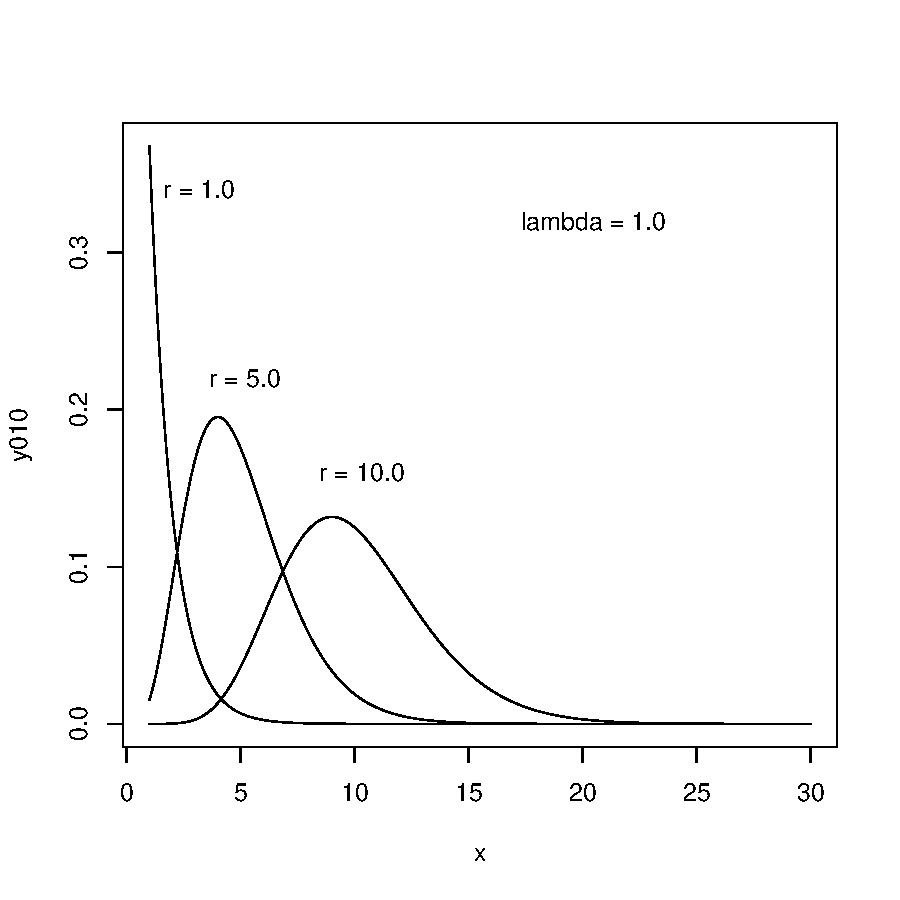
\includegraphics[width=5.0in]{Gamma.pdf}
}
\caption{Various Gamma Densities}
\label{gammas}
\end{figure}

As you might guess from the network performance analysis example in
Section \ref{netbuff}, the gamma family does arise often in the network
context, and in queuing analysis in general.

\subsection{The Beta Family of Distributions}
\label{betafamily}

As seen in Figure \ref{gammas}, the gamma family is a good choice to
consider if our data are nonnegative, with the density having
a peak near 0 and then gradually tapering off to the right.  What about
data in the range (0,1)?  

For instance, say trucking company transports many things, including
furniture.  Let $X$ be the proportion of a truckload that consists of
furniture.  For instance, if 15\% of given truckload is furniture, then
X = 0.15.  So here we have a distribution with support in (0,1).  The
beta family provides a very flexible model for this kind of setting,
allowing us to model many different concave up or concave down curves.

\subsubsection{Density Etc.}

The densities of the family have the following form:

\begin{equation}
\frac{\Gamma(\alpha+\beta)}{\Gamma(\alpha) \Gamma(\beta)}
t^{\alpha-1}(1-t)^{\beta-1}
\end{equation}

There are two parameters, $\alpha$ and $\beta$.  
Figures \ref{betadens0202}
and \ref{betadens2030}
show two possibilities.

\begin{figure}
\centerline{
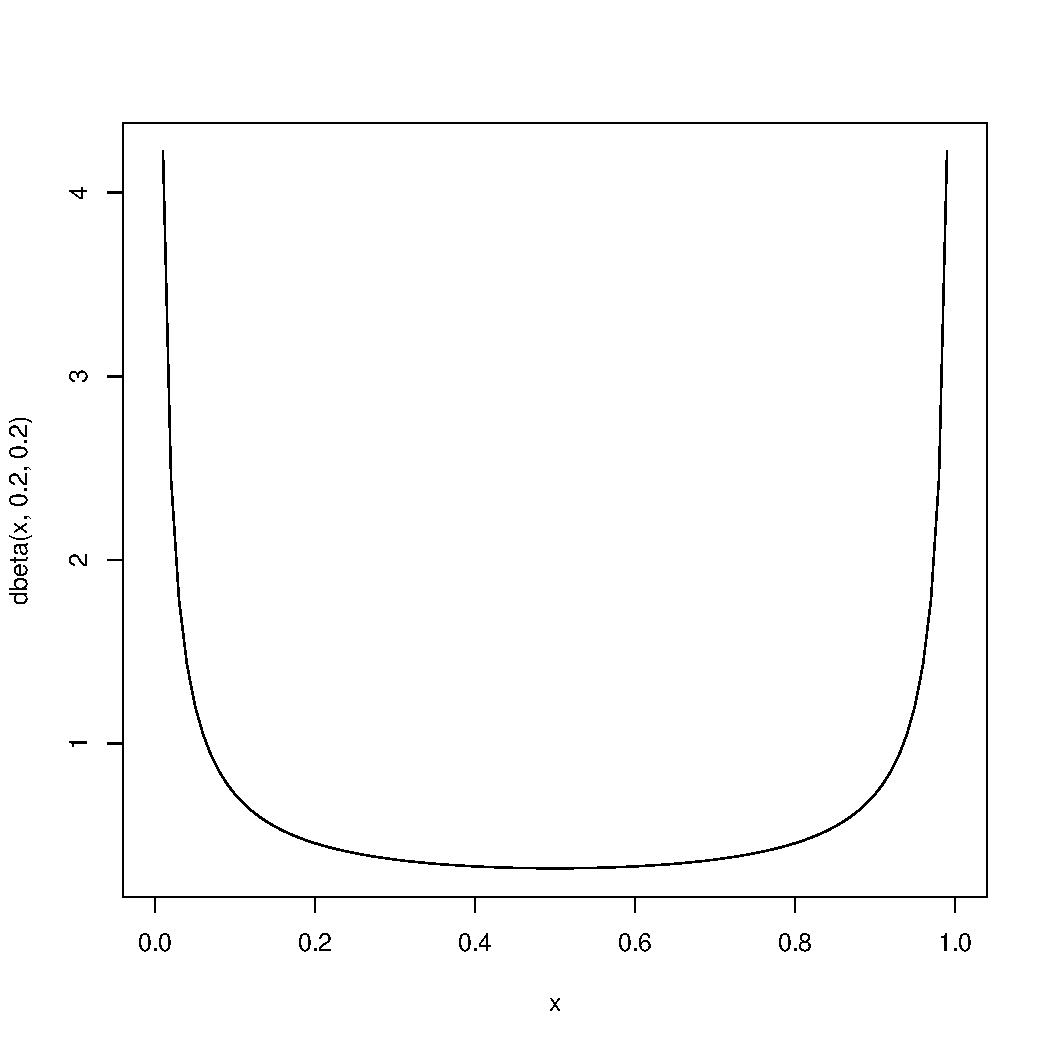
\includegraphics[width=4in]{Beta0202.pdf}
}
\caption{Beta Density, $\alpha = 0.2, \beta = 0.2$}
\label{betadens0202}
\end{figure}

\begin{figure}
\centerline{
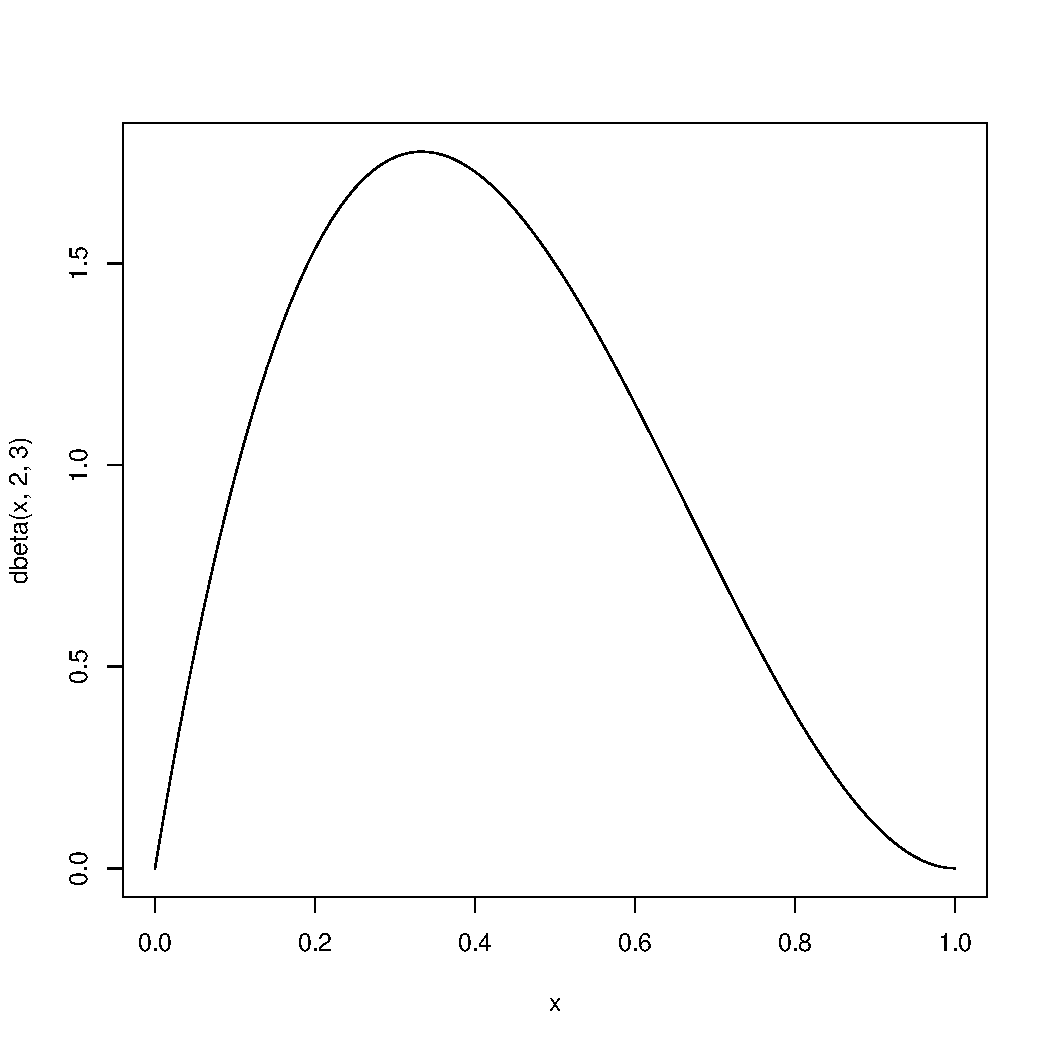
\includegraphics[width=4in]{Beta2030.pdf}
}
\caption{Beta Density, $\alpha = 2.0, \beta = 3.0$}
\label{betadens2030}
\end{figure}

% bt <- function(t) {
%    b <- gamma(alpha+beta) / (gamma(alpha) * gamma(beta)) 
%    b <- b * (1-t)^(alpha-1) * t^(beta-1)
% }
% 
% alpha <- 2
% beta <- 2
% curve(bt,0,1)
% 
% alpha <- 0.5
% beta <- 0.5
% curve(bt,0,1,add=TRUE)

The mean and variance are

\begin{equation}
\frac{\alpha}{\alpha+\beta}
\end{equation}

and

\begin{equation}
\frac
{\alpha \beta}
{(\alpha+\beta)^2 (\alpha+\beta+1)}
\end{equation}

Again, there are also {\bf dbeta()}, {\bf qbeta()} and {\bf rbeta()}.
From the R man page:

\begin{lstlisting}
Usage:

     dbeta(x, shape1, shape2, ncp = 0, log = FALSE)
     pbeta(q, shape1, shape2, ncp = 0, lower.tail = TRUE, log.p = FALSE)
     qbeta(p, shape1, shape2, ncp = 0, lower.tail = TRUE, log.p = FALSE)
     rbeta(n, shape1, shape2, ncp = 0)
\end{lstlisting}

The graphs mentioned above were generated by running

\begin{lstlisting}
> curve(dbeta(x,0.2,0.2))
> curve(dbeta(x,2,3)
\end{lstlisting}


\subsubsection{Importance in Modeling}

As mentioned, the beta family is a natural candidate for modeling a
variable having range the interval (0,1).

This family is also popular among {\bf Bayesian} statisticians
(Section \ref{bayesian}).

\section{Choosing a Model}

The parametric families presented here are often used in the real world.
As indicated previously, this may be done on an empirical basis.  We
would collect data on a random variable X, and plot the frequencies of
its values in a histogram.  If for example the plot looks roughly like
the curves in Figure \ref{gammas}, we could choose this as the family
for our model.

Or, our choice may arise from theory.  If for instance our knowledge of
the setting in which we are working says that our distribution is
memoryless, that forces us to use the exponential density family.

In either case, the question as to which member of the family we choose
will be settled by using some kind of procedure which finds the
member of the family which best fits our data.  We will discuss this in
detail in our chapters on statistics, especially Chapter \ref{chap:mod}.

Note that we may choose not to use a parametric family at all.  We may
simply find that our data does not fit any of the common parametric
families (there are many others than those presented here) very well.
Procedures that do not assume any parametric family are termed {\bf
nonparametric}.

\section{Finding the Density of a Function of a Random Variable}
\label{densgofx}

Suppose X has, say, a uniform distribution on (1,4).  Form a new random
variable, $Y = X^2$.  How can we find $f_Y()$?  Reason as follows.  For
$1 < t < 16$,

\begin{eqnarray}
f_Y(t) &=& \frac{d}{dt} F_Y(t) ~~ \textrm{(def. of density)}\\ 
&=& \frac{d}{dt} P(Y \leq t) ~~ \textrm{(def. of cdf)} \\
&=& \frac{d}{dt} P(X \leq \sqrt{t}) ~~ \textrm{(def. of Y)} \\
&=& \frac{d}{dt} F_X(\sqrt{t}) ~~ \textrm{(def. of cdf)} \\
&=& f_X(\sqrt{t}) ~ \frac{d}{d} \sqrt{t} ~~ \textrm{(Chain Rule)} \\
&=& \frac{1}{3} \cdot \frac{1}{2} t^{-0.5} \\
&=& \frac{1}{6} t^{-0.5}
\end{eqnarray}

Other such settings can be handeled similarly.  Note, though, that the
above derivation relied on the fact that $X > 0$.  Suppose X has a
uniform distribution on (-1,1).  Then the above derivation would become,
for $0 < t < 1$,

\begin{eqnarray}
f_Y(t) &=& \frac{d}{dt} P(Y \leq t) \\
&=& \frac{d}{dt} P(-\sqrt{t} \leq X \leq \sqrt{t}) \\
&=& \frac{d}{dt} 2 \sqrt{t} / 2 \\
&=& 0.5 t^{-0.5}
\end{eqnarray}

\section{Quantile Functions}

First, recall the definition of the {\bf inverse} of a function, say
$h()$.  The inverse of $h()$, denoted $h^{-1}()$, ``brings you back to
where you started.'' If I plug 3 into the squaring function, I get 9,
and if I then plug 9 into the square root function, I get back my
original 3.\footnote{This assumes, of course, that the domain of my
squaring function consists only of the nonnegative numbers.  We'll put
aside this and similar situations for the time being, but will return.}
So we say that $h(t) = t^2$ and $k(s) = \sqrt{s}$ are inverses of each
other.  The same relation holds between $\exp()$ and $\ln()$ and so on.

For a random variable X, its {\bf quantile function} $Q_X(s)$ is defined
by

\begin{equation}
Q_X(s) = F_X^{-1}(s)
\end{equation}

This is called the {\bf s quantile} of X.

A well-known example is the {\bf median} of X, the point which half
the probability is above and half below.  It's the 0.5 quantile of X.

The cdf tells us that cumulative probability for a particular value of
X, while the quantile function does the opposite, ``bringing us back.''
Let's make this concrete by considering the random variable Z in Section
\ref{cdfdef}.

On the one hand, we can ask the question, ``What is the probability that
Z is at most 1?'', with the answer being

\begin{equation}
F_Z(1) = 0.75 
\end{equation}

On the other hand, one can ask conversely, ``At what value of X do we
have cumulative probability of 0.75?''  Here the answer is

\begin{equation}
Q_Z(0.75) = 1
\end{equation}

It is no coincidence that the word {\it quantile} has that 
{\it -ile} suffix, given your familiarity with the word {\it
percentile}.  They are really the same thing.

Suppose for example that 92\% of all who take the SAT Math Test have
scores of at most 725.  In other words, if you look at a randomly chosen
test paper, and let X denote its score, then

\begin{equation}
F_X(725) = P(X \leq 725) = 0.92
\end{equation}

On the other hand, if you are interested in the 92$nd$ percentile score
for the test, you are saying ``Find s such that $P(X \leq s) = 0.92$'' you
want

\begin{equation}
Q_X(0.92) = 725
\end{equation}

The reader should note that the R functions we've seen beginning with
the letter 'q', such as {\bf qgeom()} and {\bf qunif()}, are quantile
functions, hence the name.

However, a problem with discrete random variables is that the quantile
values may not be unique.  The reader should verify, for instance, in
the coin-toss example above, the 0.75 quantile for Z could be not only
1, but also 1.1, 1.288 and so on.  So, one should look carefully at the
documentation of quantile functions, to see what they do to impose
uniqueness.  But for continuous random variables there is no such
problem.

\section{Using cdf Functions to Find Probabilities}

As we have seen, for many parametric families R has ``d/p/q/r''
functions, giving the density, cdf, quantile function and random number
generator for the given family.  How can we use the cdf functions to
find probabilities of the form $P(a < X < b)$?

We see the answer in (\ref{ntab}).  We simply evaluate the cdf at $b$
then $a$, and subtract.

For instance, consider the network buffer example, Section
\ref{netbuff}.  Let's find $P(540 < Y < 562)$:

\begin{lstlisting}
> pgamma(562,5,0.01) - pgamma(540,5,0.01)
[1] 0.03418264
\end{lstlisting}

Of course, we could also integrate the density,

\begin{lstlisting}
> integrate(function(t) dgamma(t,5,0.01),540,562)
0.03418264 with absolute error < 3.8e-16
\end{lstlisting}

but R does that for us, there is probably little point in that second
approach.

\section{A General Method for Simulating a Random Variable}
\label{genrannumgen}

Suppose we wish to simulate a random variable X with density $f_{X}$ for
which there is no R function. This can be done via $F_X^{-1}(U)$, where
U has a U(0,1) distribution.  In other words, we call {\bf runif()} and
then plug the result into the inverse of the cdf of X. 

For example, say X has the density 2t on (0,1). Then $F_X(t) = t^2$, so
$F^{-1}(s) = s^{0.5}$.  We can then generate an X as {\bf
sqrt(runif(1))}.  Here's why:

For brevity, denote $F_X^{-1}$ as G.  Our generated random variable is
then Y = G(U).  Then

\begin{eqnarray}
F_Y(t) &=& P[G(U)\leq t] \\
& = & P[U\leq G^{-1}(t)] \\
& = & P[U\leq F_X(t)] \\
& = & F_X(t)
\end{eqnarray}

(this last coming from the fact that U has a uniform distribution on
(0,1)).

In other words, Y and X have the same cdf, i.e.\ the same distribution!
This is exactly what we want.

Note that this method, though valid, is not necessarily practical, since
computing $F_X^{-1}$ may not be easy.

\section{Example:  Writing a Set of R Functions for a Certain Power Family}

Consider the family of distributions indexed by positive values of
{\it c} with densities

\begin{equation}
c ~ t^{c-1}
\end{equation}

for t in (0,1) and 0 otherwise..

The cdf is $t^c$, so let's call this the ``tc'' family.

Let's find ``d'', ``p'', ``q'' and ``r'' functions for this family, just
like R has for the normal family, the gamma family and so on:

\begin{lstlisting}
# density
dtc <- function(x,c) c * x^(c-1)

# cdf
ptc <- function(x,c) x^c

# quantile function
qtc <- function(q,c) q^(1/c)

# random number generator, n values generated
rtc <- function(n,c) {
   tmp <- runif(n)
   qtc(tmp,c)
}
\end{lstlisting}

Note that to get {\bf rtc()} we simply plug U(0,1) variates into {\bf
qtc()}, according to Section \ref{genrannumgen}.

Let's check our work.  The mean for the density having {\it c} equal to
2 is 2/3 (reader should verify); let's see if a simulation will give us
that:

\begin{lstlisting}
> mean(rtc(10000,2))
[1] 0.6696941
\end{lstlisting}

Sure enough!

\section{Multivariate Densities}
\label{minimulcontin}

Section \ref{minimul} briefly introduced the notion of multivariate
pmfs.  Similarly, there are also multivariate densities.  Probabilities
are then k-fold integrals, where k is the number of random variables. 

For instance, a probability involving two variables means taking a
double integral of a bivariate density.  Since that density can be
viewed as a surface in three-dimensional space (just as a univariate
density is viewed as a curve in two-dimensional space), a probability is
then a volume under that surface (as opposed to area in the univariate
case).  Conversely, a bivariate density is the mixed partial derivative
of the cdf:

\begin{equation}
f_{X,Y} (u,v) = \frac{\partial^2}{\partial u \partial v}
F_{X,Y}(u,v) = P(X \leq u, ~ Y \leq v)
\end{equation}

In analogy to

\begin{equation}
P(B ~|~ A) = \frac{P(B \textrm{ and } A)}{P(A)}
\end{equation}

we can define the conditional density of Y given X:

\begin{equation}
f_{Y|X} (u,v) =
\frac{f_{X,Y} (u,v)}{f_X(v)}
\end{equation}

The intuition behind this is that we are conditioning on X being {\it
near} v.  Actually, 

\begin{equation}
f_{Y|X} (u,v) =
\lim_{h \rightarrow 0} ~
\left [
\textrm{density of Y} ~|~ X \in (v-h,v+h)
\right ]
\end{equation}

A detailed treatment is presented in Chapter \ref{mul}.

% \section{``Hybrid'' Continuous/Discrete Distributions}
% \label{mixed}
% 
% A random variable could have a distribution that it partly discrete and
% partly continuous.  Recall our first example, from Section \ref{dart},
% in which D is the position that a dart hits when thrown at the interval
% (0,1).  Suppose our measuring instrument is broken, and registers any
% value of D past 0.8 as being equal to 0.8.  Let W denote the actual
% value recorded by this instrument.  
% 
% Then P(W = 0.8) = 0.2, so W is not a continuous random variable, in
% which every point has mass 0.  On the other hand, P(W = t) = 0 for every
% t before 0.8, so W is not discrete either.
% 
% In the advanced theory of probability, some very odd mixtures, beyond
% this simple discrete/continuous example, can occur, though primarily of
% theoretical interest.

\section{Iterated Expectations}

In analogy with (\ref{adamsdiscrete}), we have a very useful
corresponding formula for the continuous case.

\subsection{The Theorem}

For any random variable W and any continuous random variable
V,\footnote{The treatment here will be intuitive, rather than being a
mathematical definition and proof.}

\begin{equation}
\label{adamscontin}
E(W) = \int_{-\infty}^{\infty} f_V(t) ~ E(W ~|~ V = t)~ dt
\end{equation}

Note that the event $V ~=~ t$ has probability 0 for coninuous V.  The
conditional expectation here is defined in terms of the conditional
distribution of W given V; see Section \ref{minimulcontin}.

Note too that if we have some event A, we can set W above to the
indicator random variable of A (recall (\ref{indicator})), yielding

\begin{equation}
\label{adamscontinprob}
P(A) = \int_{-\infty}^{\infty} f_V(t) ~ P(A ~|~ V = t)~ dt
\end{equation}

\subsection{Example:  Another Coin Game}

Suppose we have biased coins of various weightings, so that a randomly
chosen coin's probability of heads H has density 2t on (0,1).  The game
has you choose a coin at random, toss it 5 times, and pays you a prize
if you get 5 heads.  What is your probability of winning?

First, note that the probability of winning, given H = t, is $t^5$.
then (\ref{adamscontinprob}) tells us that

\begin{equation}
P(\textrm{win}) = \int_{0}^{1} 2t ~ t^5   ~ dt = \frac{2}{7}
\end{equation}

\section{Continuous Random Variables Are ``Useful Unicorns''}
\label{unicorns}

Recall our random dart example at the outset of this chapter.  It must
be kept in mind that this is only an idealization.  D actually cannot be
just any old point in (0,1).  To begin with, our measuring instrument
has only finite precision.  Actually, then, D can only take on a finite
number of values.  If, say, our precision is four decimal digits, then D
can only be 0.0001, 0.0002, ...,  0.9999, making it a discrete random
variable after all.\footnote{There are also issues such as the nonzero
thickness of the dart, and so on, further restricting our measurement.}

So this modeling of the position of the dart as continuously distributed
really is just an idealization.  {\it Indeed, in practice there are NO
continuous random variables.}  But the coninuous model can be an
excellent approximation, and the concept is extremely useful.  It's like
the assumption of ``massless string'' in physics analyses; there is no
such thing, but it's a good approximation to reality.

As noted, most applications of statistics, and many of probability, are
based on continuous distributions.  We'll be using them heavily for the
remainder of this book.

